\chapter{Estado del Arte}
\section{Aplicaciones Similares}

Existen múltiples aplicaciones diseñadas para facilitar la búsqueda de eventos y establecimientos sociales. Por
ejemplo, aplicaciones como Yelp, Google y TripAdvisor permiten a los usuarios buscar restaurantes, bares, y eventos
según las reseñas y valoraciones de otros usuarios.

\begin{enumerate}
    \item \textbf{TripAdvisor:} Tripadvisor es la plataforma de orientación de viajes más grande del mundo. Ayuda a
          cientos de millones de personas cada mes en la planificación, reserva y realización de viajes. Los viajeros usan
          el sitio y la aplicación para descubrir alojamientos, actividades y restaurantes basados en las recomendaciones
          de otros viajeros.\cite{tripadvisor}

    \item \textbf{Yelp:} Yelp conecta a las personas con excelentes negocios locales. Con información confiable
          sobre negocios locales, fotos y contenido de reseñas, Yelp proporciona una plataforma local integral para que
          los consumidores descubran, se conecten y realicen transacciones con negocios de todos los tamaños, facilitando
          la solicitud de presupuestos, la unión a listas de espera, la realización de reservas y la programación de citas
          o compras.\cite{yelp}

    \item \textbf{Google:} Google Maps permite a los turistas descubrir una amplia variedad de establecimientos de
          ocio, como restaurantes, bares, parques, museos y otros puntos de interés. La función de búsqueda integrada
          facilita encontrar lugares específicos o explorar categorías de interés en una zona determinada.\cite{google}

\end{enumerate}

A continuación, se muestran imágenes de las aplicaciones mencionadas para su mejor visualización:

\begin{figure}[H]
    \centering

    \begin{subfigure}{.3\textwidth}
        \centering
        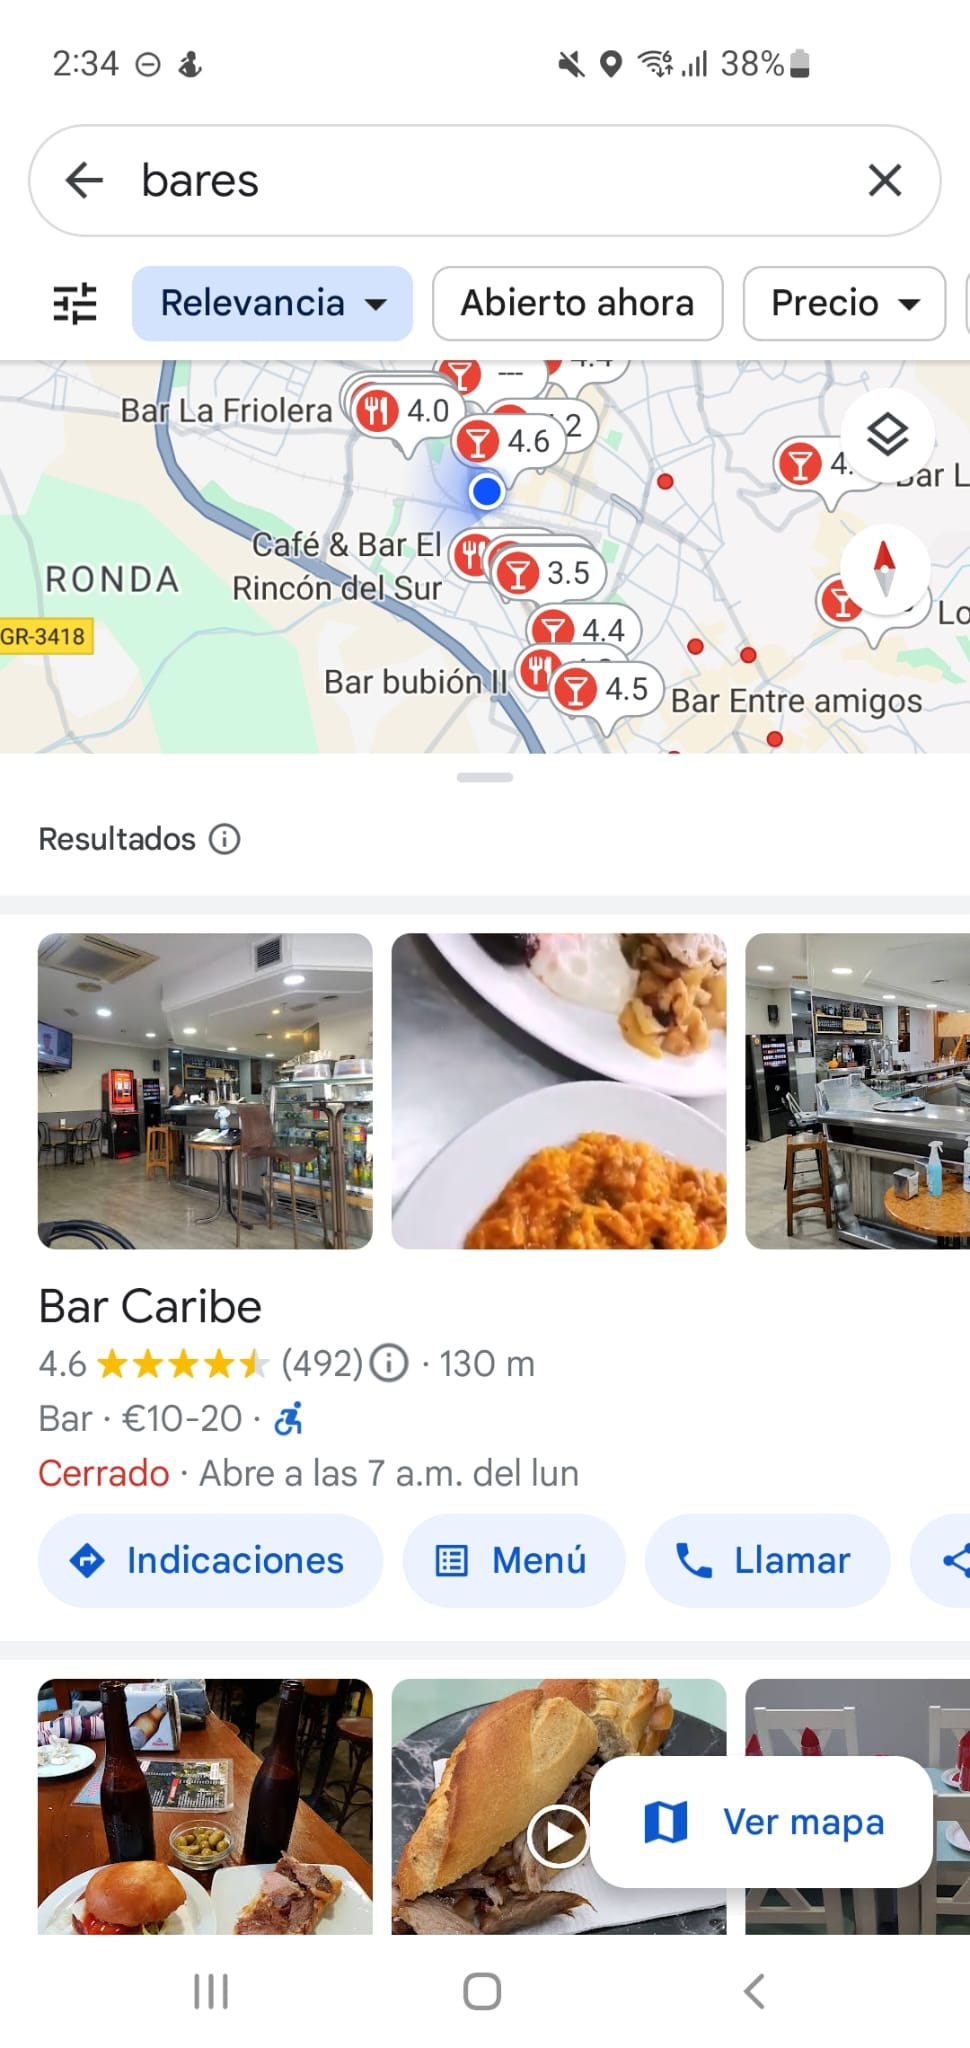
\includegraphics[width=\linewidth]{imagenes/GoogleMaps.jpeg}
        \caption{Google Maps}
        \label{fig:img1}
    \end{subfigure}%
    \hfill
    \begin{subfigure}{.3\textwidth}
        \centering
        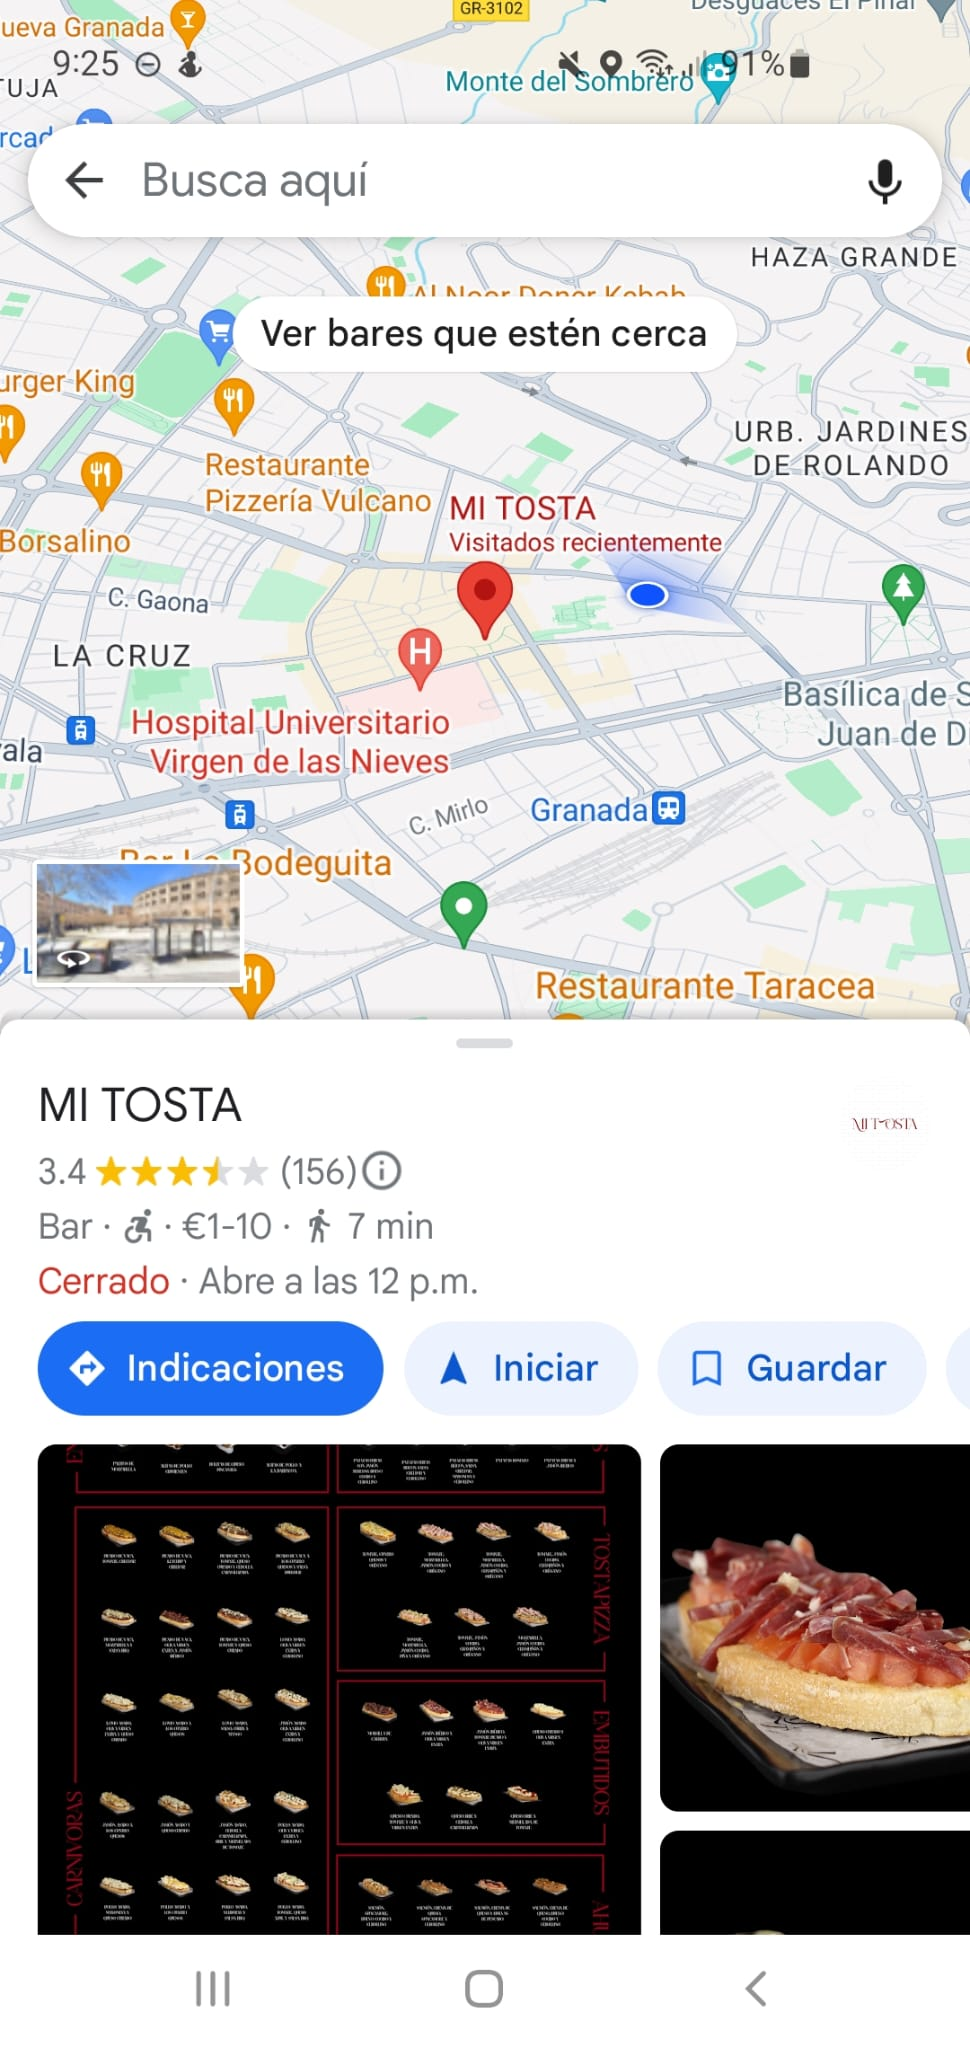
\includegraphics[width=\linewidth]{imagenes/Maps.jpeg}
        \caption{Google Maps}
        \label{fig:img2}
    \end{subfigure}%
    \hfill
    \begin{subfigure}{.3\textwidth}
        \centering
        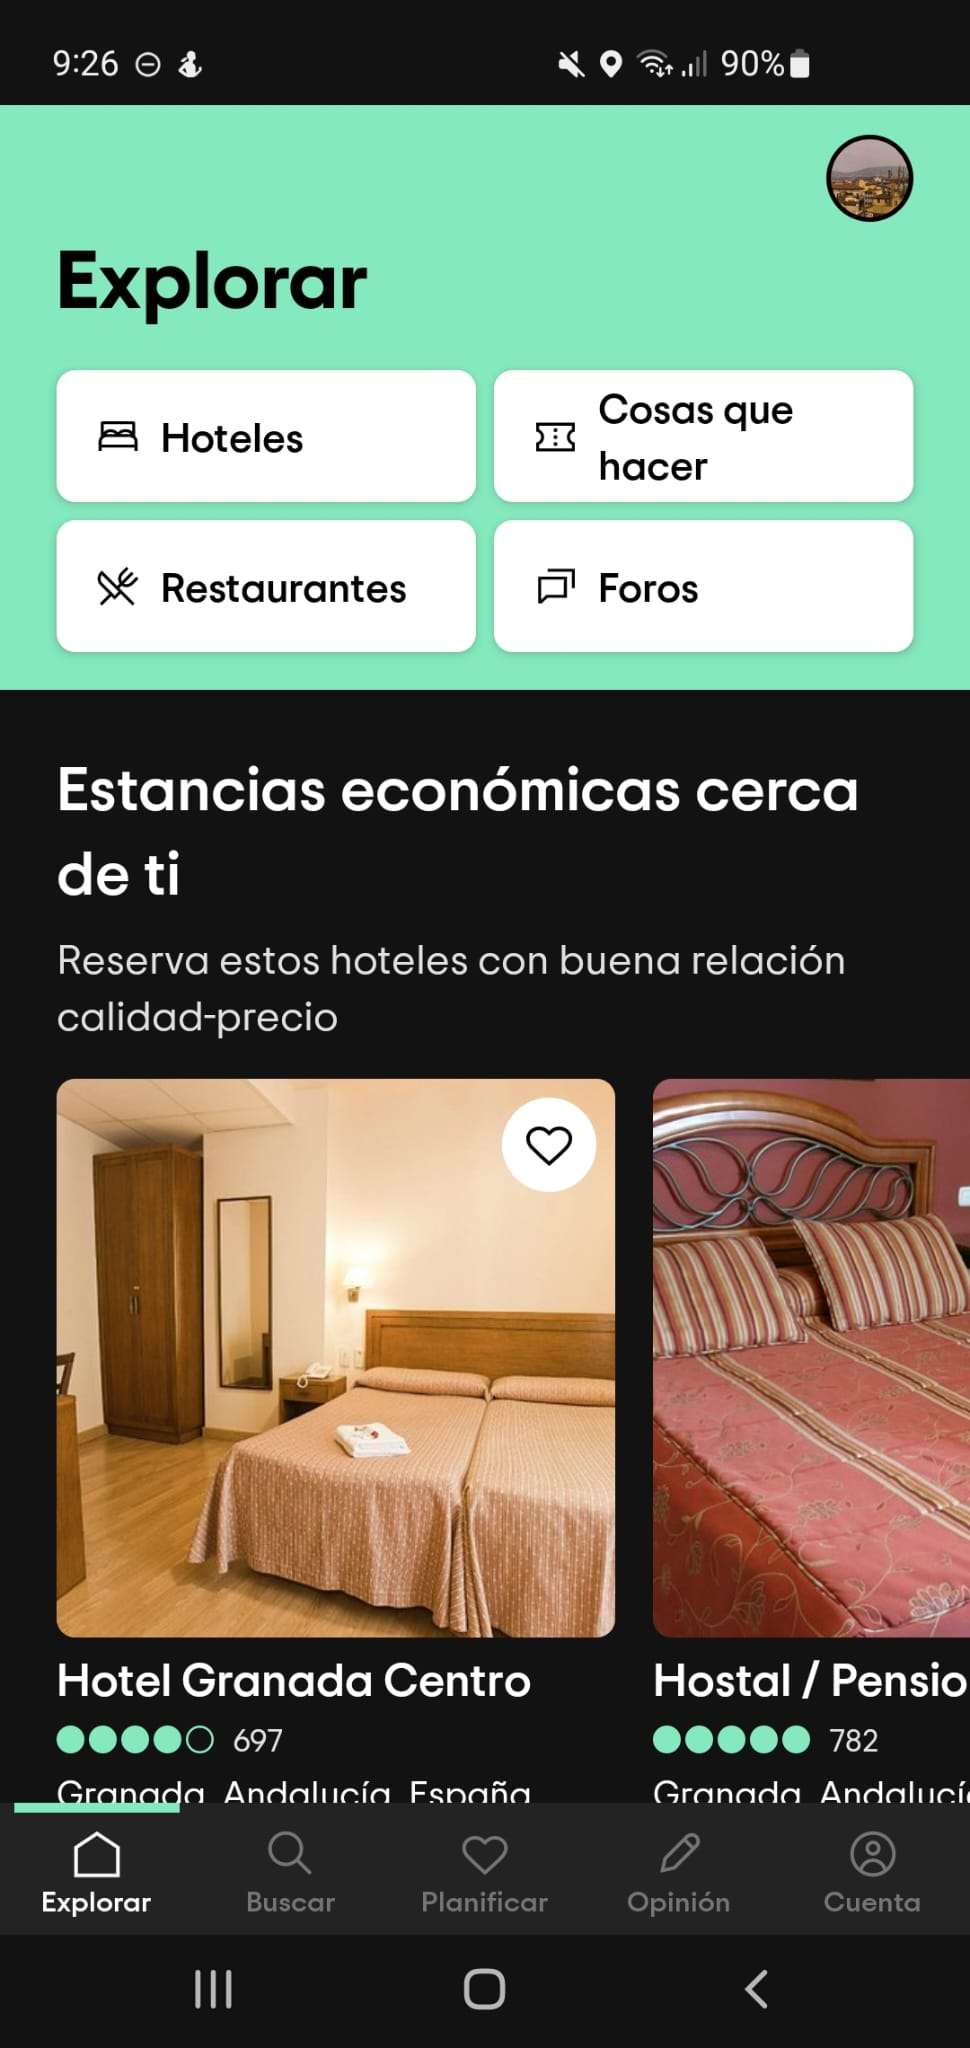
\includegraphics[width=\linewidth]{imagenes/TripAdvisor1.jpeg}
        \caption{TripAdvisor}
        \label{fig:img3}
    \end{subfigure}

    \vspace{1em}

    \begin{subfigure}{.3\textwidth}
        \centering
        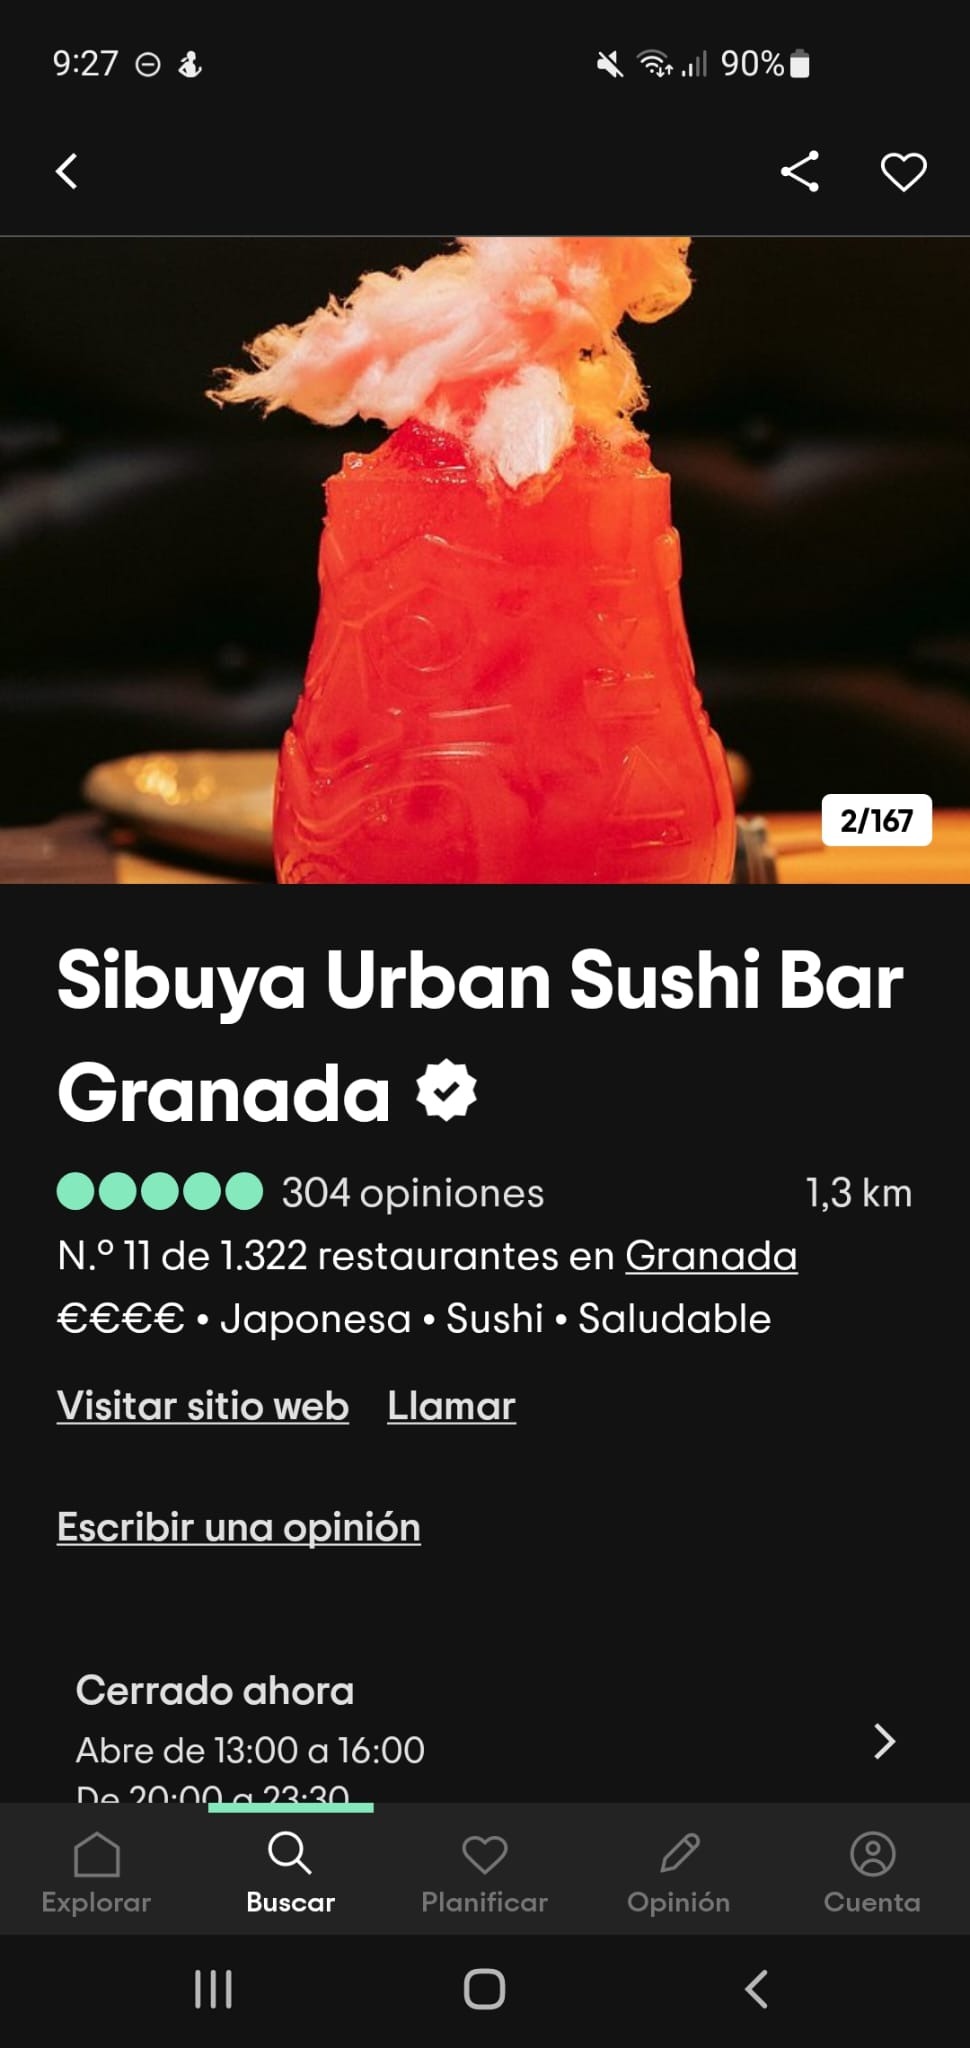
\includegraphics[width=\linewidth]{imagenes/TripAdvisor2.jpeg}
        \caption{TripAdvisor}
        \label{fig:img4}
    \end{subfigure}%
    \hfill
    \begin{subfigure}{.3\textwidth}
        \centering
        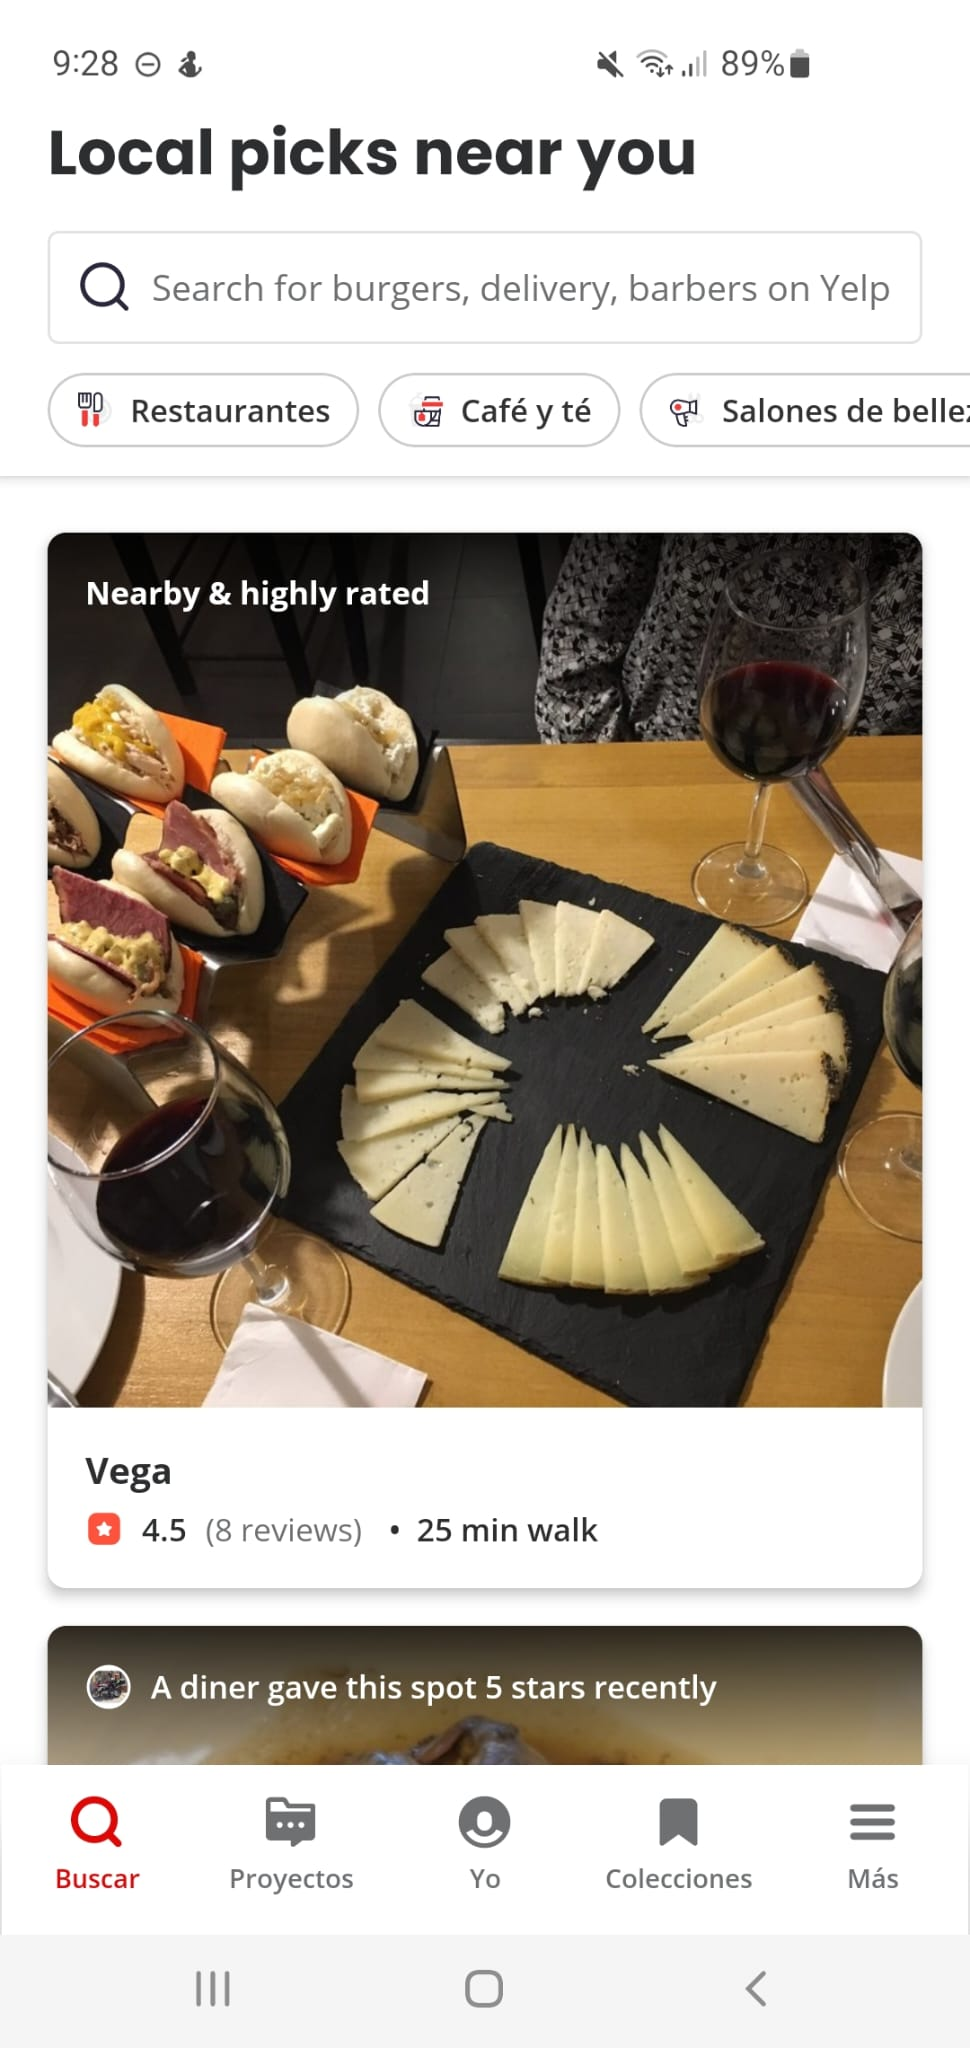
\includegraphics[width=\linewidth]{imagenes/Yelp1.jpeg}
        \caption{Yelp}
        \label{fig:img5}
    \end{subfigure}%
    \hfill
    \begin{subfigure}{.3\textwidth}
        \centering
        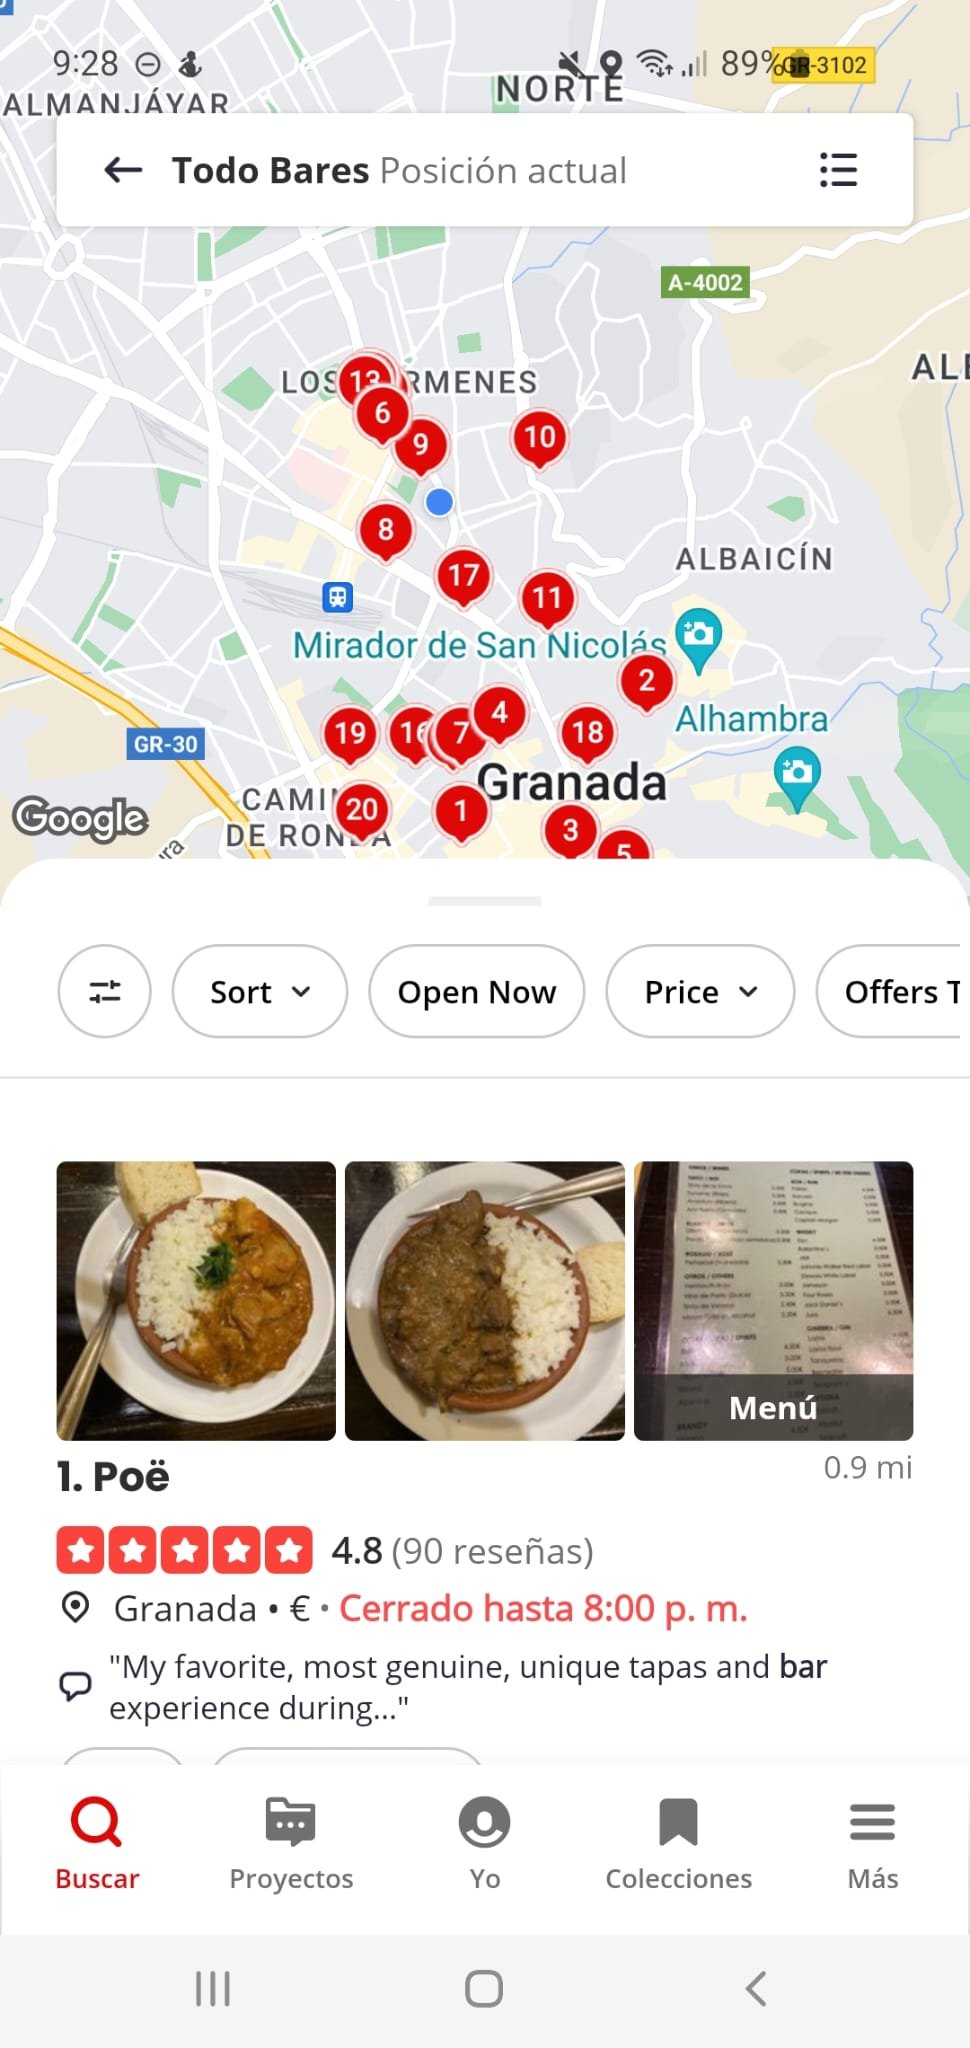
\includegraphics[width=\linewidth]{imagenes/Yelp2.jpeg}
        \caption{Yelp}
        \label{fig:img6}
    \end{subfigure}

    \caption{Comparación de aplicaciones orientadas al turismo}
    \label{fig:comparacion_apps}
\end{figure}

Estas aplicaciones aunque sean excelentes en muchos aspectos tienen ciertas limitaciones como pueden ser:

\begin{enumerate}

    \item \textbf{Información Fragmentada:} Los usuarios deben de consultar distintas plataformas y seguir a
          diversos establecimientos en sus redes sociales para estar al tanto de eventos u ofertas, lo que resulta en una
          experiencia fragmentada. Esta dispersión no es sólo ineficiente, sino que puede llevar a que los usuarios
          pierdan el interés y abandonen la búsqueda con consecuencia que pierdan una oportunidad importante de encontrar
          ese lugar que buscan.

    \item \textbf{Interacción Social Limitada:} Estas aplicaciones permiten leer reseñas y calificaciones en un
          establecimiento por parte de otros usuarios pero no permiten la creación de actividades entre amigos ni fomentan
          la organización y la interacción social.

    \item \textbf{Promoción y Gestión para Establecimientos:} La gestión de los perfiles y la promoción de eventos y
          ofertas en estas plataformas no es una prioridad. Estas aplicaciones tienden a centrarse más en la experiencia
          del usuario, ofreciendo calificaciones y reseñas de los establecimientos, pero no promueven activamente los
          lugares con los eventos y ofertas que pueden tener.

    \item \textbf{Enfoque Amplio y no Exclusivo al Ocio:} Estas aplicaciones abarcan un conjunto de funcionalidades
          no exclusivamente centradas en el ocio. Por ejemplo, TripAdvisor proporciona información sobre hoteles,
          atracciones turísticas y restaurantes, mientras que Google requiere búsquedas individuales de cada
          establecimiento hasta encontrar uno que se ajuste a las necesidades del usuario.

\end{enumerate}

\section{Soluciones HangOut}

Para solucionar estas limitaciones se ha desarrollado HangOut, una aplicación móvil diseñada para asistir a las personas para encontrar un establecimiento o evento adecuado a sus gustos que integra y mejora las funcionalidades existentes con características innovadoras:


\begin{enumerate}
    \item \textbf{Centralización de la Información:} HangOut centraliza la información de diversos establecimientos y eventos, permitiendo al usuario encontrar rápidamente opciones que se ajusten a sus preferencias sin necesidad de consultar múltiples fuentes.

    \item \textbf{Interacción y Organización Social:} La aplicación permite a los usuarios seguir a otros, crear actividades y organizar salidas grupales de manera más eficiente, eliminando la necesidad de coordinarse a través de múltiples aplicaciones de mensajería.

    \item \textbf{Herramientas para Administradores de Establecimiento:} HangOut proporciona a los administradores una plataforma para gestionar sus perfiles de establecimiento indicando el ambiente, eventos y ofertas, facilitando así la promoción y gestión de sus servicios de manera más eficaz.

    \item \textbf{Enfoque Exclusivo:} La aplicación se distingue por su enfoque exclusivo en el ocio y la eficiencia en la organización de eventos. Combinando la funcionalidad de creaciones de actividades en grupos específicos con la búsqueda de establecimientos y la personalización según las preferencias del usuario, ofreciendo una solución más específica para el ocio.
\end{enumerate}

\begin{table}[H]
    \centering
    \label{tab:comparison}
    \small
    \begin{tabularx}{\textwidth}{|X|X|X|X|X|X|}
        \hline
                                               & \textbf{TripAdvisor} & \textbf{Yelp} & \textbf{Google Maps} \\ \hline
        \textbf{Búsqueda por Filtros}          & Si                   & Si            & Si                   \\ \hline
        \textbf{Centralizado}                  & Si                   & Si            & Si                   \\ \hline
        \textbf{Exclusivo}                     & No                   & No            & No                   \\ \hline
        \textbf{Organización Social}           & No                   & No            & No                   \\ \hline
        \textbf{Promoción de Establecimientos} & Si                   & No            & No                   \\ \hline
    \end{tabularx}
    \caption{Comparación de características de aplicaciones para el turismo}

\end{table}


